% -----------------------------------------------------------------------------
% IMPORTANT NOTICE:\clearpage\chapter{Chapter Title Here}


% This LaTeX document template is provided by Dr. Girish Kumar N G, Assistant Professor 
%Department of Electronics and Telecommunication Engineering
%Bangalore Institute of Technology, V V Pura, K R Road, Bengaluru-560004.
% It is intended for educational purposes and for use by students
% in preparing their reports. All rights to the original template
% remain reserved by the author. 
%
% Students are permitted to edit and customize this template for
% their reports; however, the original authorship and attribution 
% must not be removed or altered.
%
% Any unauthorized distribution, reproduction, or commercial use
% of this template, in part or in whole, is strictly prohibited 
% without prior written consent from the author.
% -----------------------------------------------------------------------------

%contents that you see in blue colour and brackets, symbols in red  are coding commands do not edit it until you know coding and feel to edit

\documentclass[12pt]{report}% document starts from here with standard document class
\documentclass[openany]{book}

% Package imports- these are package imports dont edit these packages
\usepackage{graphicx} % For including graphics
\usepackage{geometry} % For adjusting page margins
\usepackage{fancyhdr} % For headers and footers
\usepackage{mdframed} % For creating page borders
\usepackage{setspace} % For line spacing
\usepackage{tocloft} % For formatting TOC, LOF, and LOT
\usepackage{tabularx}
\usepackage{float} % For the H option in figure floats
\usepackage{algorithm}
\usepackage{algpseudocode} % For the algorithmic environment
\usepackage{nomencl} % For abbreviations list
\usepackage{etoolbox} % Needed for \patchcmd
\usepackage{ragged2e}
\usepackage{longtable}
\usepackage{url}      % for \url command in bibliography
\usepackage[hidelinks]{hyperref}
\usepackage{hyperref} % optional, for clickable links
\usepackage{titlesec}  % Add this package
\usepackage{caption}

\titlespacing*{\chapter}{0pt}{-40pt}{10pt} % Reduce space before chapter heading

% Fix: Unicode subscript 2 (₂) in SpO₂ when compiling with pdfLaTeX
\DeclareUnicodeCharacter{2082}{\textsubscript{2}}
% ------------------------------------------------------------
% GLOBAL SPACING BETWEEN TABLE/FIGURE AND TEXT
% ------------------------------------------------------------
\setlength{\intextsep}{4pt}   % Default ~8pt, increase to add 2–3 mm space

\usepackage{titlesec}

% Customize chapter heading: Chapter 1 Introduction (on the same line)
\makeatletter
\def\@makechapterhead#1{%
  \vspace*{-25pt}% Adjust space before chapter number
  {\parindent \z@
    \raggedright
    \normalfont
    \fontsize{16pt}{20pt}\selectfont\bfseries
    Chapter \thechapter\par\nobreak
    \vskip 8pt
    \begin{center}
      \fontsize{20pt}{22pt}\selectfont\bfseries #1
    \end{center}
    \vskip 2pt
  }}
\def\@makeschapterhead#1{%
  \vspace*{-25pt}%
  {\parindent \z@
    \normalfont
    \fontsize{20pt}{22pt}\selectfont\bfseries
    \begin{center}#1\end{center}\par\nobreak
    \vskip 5pt
  }}
\makeatother

% ------------------------------------------------------------
% SECTION AND SUBSECTION FONT SIZE FORMATTING
% ------------------------------------------------------------
\titleformat{\section}
  {\normalfont\fontsize{16pt}{20pt}\bfseries}
  {\thesection}{1em}{}

\titleformat{\subsection}
  {\normalfont\fontsize{14pt}{18pt}\bfseries}
  {\thesubsection}{1em}{}

\makenomenclature
\geometry{a4paper, left=1.25in, right=1in, top=1in, bottom=1in}


% dont edit these- the below codes are written to give page numbers roman numbers for preliminary pages and arabic numbering for content pages

\fancypagestyle{preliminary}{
    \fancyhf{}
    \fancyfoot[C]{\thepage} % Center Roman page numbers
    \setlength{\footskip}{0.75in}
    \renewcommand{\headrulewidth}{0pt}
    \renewcommand{\footrulewidth}{0pt}
}
% dont edit these- the below codes are written to give page numbers roman numbers for preliminary pages and arabic numbering for content pages

\fancypagestyle{maincontent}{
    \fancyhf{}
    \fancyfoot[C]{\thepage} % Center Arabic page numbers
    \setlength{\footskip}{0.75in}
    \renewcommand{\headrulewidth}{0pt}
    \renewcommand{\footrulewidth}{0pt}
}
\makeatletter
\patchcmd{\chapter}
  {\thispagestyle{plain}} % Replace plain style
  {\thispagestyle{maincontent}} % Apply the custom style
  {}{} % Do nothing if the patch fails
\makeatother

\fancypagestyle{maincontent}{
    \fancyhf{} % Clear all header and footer fields

    % Header
    \fancyhead[L]{\textbf{ResQNow: AI-AR First Aid \& Emergency App}} % Left side of header
    \fancyhead[R]{\textbf{2025-2026}} % Right side of header
    \renewcommand{\headrulewidth}{1.5pt} % Thickness of header line
    \renewcommand{\headrule}{%
        \hrule height 1.5pt % Top border thickness
        \vspace{1pt} % Small gap
        \hrule height 0.5pt % Bottom border thickness
    }

  % Footer
\fancyfoot[L]{\textbf{Dept. of CSE(ICB), BIT}} % Left side of footer
\fancyfoot[R]{\thepage} % Right side of footer
\renewcommand{\footrulewidth}{1.5pt} % Top border thickness
\renewcommand{\footrule}{%
    \vspace{-3pt}% move rule a bit up
    \hrule height 1.5pt
    \vspace{0.5pt}
    \hrule height 0.5pt
    \vspace{2pt} % adjust as needed
    }
}


% Table caption spacing (unchanged)
\setlength{\belowcaptionskip}{8pt}
\captionsetup[table]{skip=8pt}

% Figure caption spacing (reduced)
\captionsetup[figure]{skip=4pt}

% Space between figure and following text/section
\setlength{\textfloatsep}{6pt}


% ------------------------------------------------------------
% Reduce space ABOVE titles of TOC, LOF, LOT ONLY
% (Does NOT affect chapters or section headings)
% ------------------------------------------------------------

% Table of Contents
\setlength{\cftbeforetoctitleskip}{-0.4cm}

% List of Figures
\setlength{\cftbeforeloftitleskip}{-0.4cm}

% List of Tables
\setlength{\cftbeforelottitleskip}{-0.4cm}


\begin{document}

% Title Page (No page number)-from here the title page code begins kindly see the content where to edit

% -----------------------------------------------------------------------------
% TITLE PAGE (REPLACED WITH UPDATED BIT / VTU FORMAT)
% -----------------------------------------------------------------------------
\begin{titlepage}
    \begin{mdframed}[linewidth=3pt, innerleftmargin=10pt, innerrightmargin=10pt, innertopmargin=10pt, innerbottommargin=10pt]
        \begin{center}
            \textbf{\fontsize{14pt}{16pt}\selectfont VISVESVARAYA TECHNOLOGICAL UNIVERSITY}\\[0.2cm]
            \textbf{\fontsize{14pt}{16pt}\selectfont BELAGAVI-590018}\\[0.3cm]
            
            % VTU LOGO
            \includegraphics[width=0.22\textwidth,keepaspectratio]{VTU.png}\\[0.3cm]
            
            \textbf{\fontsize{14pt}{16pt}\selectfont Project Report On}\\[0.3cm]
            \textbf{\fontsize{14pt}{18pt}\selectfont
            \textcolor{black}{"ResQNow: AI-AR First Aid \& Emergency App"}}\\[0.3cm]
            
            \fontsize{12pt}{14pt}\selectfont Submitted in partial fulfillment of the requirements for the\\
            award of the Degree of\\[0.3cm]
            \textbf{\fontsize{14pt}{16pt}\selectfont Bachelor of Engineering}\\[0.2cm]
            in\\[0.2cm]
            \textbf{\fontsize{13pt}{15pt}\selectfont CSE (IoT \& Cyber Security including Blockchain Technology)}\\[0.5cm]
            
            \textbf{\fontsize{12pt}{14pt}\selectfont Submitted by}\\[0.3cm]
            \begin{tabular}{c c}
                1BI22IC001 & A P SAROON \\
                1BI22IC038 & MEDHA BHAT \\
                1BI22IC057 & SUFAILA T S \\
                1BI23IC405 & PRANAVA N A \\
            \end{tabular}\\[0.5cm]
            
            \textbf{\fontsize{12pt}{14pt}\selectfont Under the guidance of}\\[0.3cm]
            \textbf{\fontsize{12pt}{14pt}\selectfont Dr. K C Anupama}\\
            \fontsize{11pt}{13pt}\selectfont Assistant Professor\\
            \fontsize{11pt}{13pt}\selectfont Dept of CSE(ICB)\\[0.3cm]
            
            % BIT LOGO
            \includegraphics[width=0.13\textwidth,keepaspectratio]{BITlogo.png}\\[0.3cm]
            
            \textbf{\fontsize{13pt}{15pt}\selectfont BANGALORE INSTITUTE OF TECHNOLOGY}\\[0.2cm]
            \fontsize{11pt}{13pt}\selectfont K R Road, V V Pura, Bengaluru-560004\\[0.2cm]
            \fontsize{9pt}{11pt}\selectfont Affiliated to VTU, Belagavi, Approved by AICTE, Accredited by NBA, NAAC\\[0.3cm]
            
            \textbf{\fontsize{12pt}{14pt}\selectfont 2025--2026}
        \end{center}
    \end{mdframed}
\end{titlepage}


% Start Roman numbering for preliminary pages

% Project Certificate sheet begins from here, only edit where ever it is mentioned to edit

\pagenumbering{roman}
\pagestyle{preliminary}
\setcounter{page}{1}
\newpage
% Certificate
%\chapter*{Certificate}
\addcontentsline{toc}{chapter}{Certificate}
%%\begin{spacing}{1.25}
\tolerance =1
\emergencystretch=\maxdimen
\hyphenpenalty=10000
\hbadness=10000
\begin{center}
{\large\textbf{BANGALORE INSTITUTE OF TECHNOLOGY}}\\[0.2cm]
\textbf{\fontsize{11pt}{13pt}\selectfont CSE (IoT \& Cyber Security including Blockchain Technology)}
\\
{\fontsize{12pt}{14pt}\selectfont K R Road, V V Pura, Bengaluru-560004.}\\[0.5cm]
\includegraphics[width=1.5in,height=1.5in,keepaspectratio]{BITlogo} % Add your college logo
\end{center}

\begin{center}
\vspace{0.1in}
\bfseries\LARGE{CERTIFICATE}
\end{center}
\vspace{0.2in}

\begin{spacing}{1.25} % Set the line spacing to 1.25
\normalfont
\noindent

% in  below paragraph your name and USN in bracket should be mentioned in a proper Chronological order of your USN number
 This is to certify that the project report entitled \textbf{"ResQNow: AI-AR First Aid \& Emergency App"} submitted by\textbf{ A P SAROON (1BI22IC001), MEDHA BHAT (1BI22IC038), SUFAILA T S (1BI22IC057) and PRANAVA N A (1BI23IC405) } to the Visvesvaraya Technological University, Belagavi, in partial fulfillment for the award of the degree of \textbf{B.E. in Computer Science and Engineering (IoT \& Cyber Security including Blockchain Technology)} is a \textit{bonafide} record of project work carried out by them under our supervision. The contents of this report, in full or in parts, have not been submitted to any other Institution or University for the award of any degree.\\[0.4cm]
\end{spacing}
\vspace{0.65cm}

%in below part of the code you need to mention your guide and your HODs name
\begin{center}
    % \textwidth makes the table span the full width of the page
    % @{\extracolsep{\fill}} automatically adds space between columns
    % l = Left align, c = Center align, r = Right align
    \begin{tabular*}{\textwidth}{@{\extracolsep{\fill}}ccc}
    
        \textbf{Project Guide} &  & \textbf{HOD} \\[0.1cm]
    
        Dr.\ Anupama K C & & Dr.\ Shivakumar B R \\[0.1cm]
        Associate Professor &  & Professor \& HOD \\[0.1cm]
        Dept of CSE(ICB), & & Dept of CSE(ICB), \\[0.1cm]
        BIT,Bengaluru-560004 & \textbf{Principal} &  BIT,Bengaluru-560004  \\[0.1cm]
        & Dr. Shanthala S &      \\[0.1cm]
        & BIT,Bengaluru-560004&
        
    \end{tabular*}
\end{center}

% no need of editing the below further part of the code of certificate  as it is College Principal Details and examiners details

\begin{center}
\end{center}

\vspace{0.15cm}

\begin{center}
\textbf{\large{\underline{Project Final Viva Voce Examination}}}
\end{center}

\vspace{0.3cm}

\begin{center}
\begin{tabular}{|m{2.5cm}|m{10cm}|} % Using m{} for vertical and horizontal centering
		\hline
		\textbf{Examiners} & \textbf{Signature with Date} \\\hline
		\textbf{Examiner 1} & \rule{0pt}{0.75cm} \\\hline % Increased vertical space
		\textbf{Examiner 2} & \rule{0pt}{0.75cm} \\\hline % Increased vertical space
	\end{tabular}
\end{center}

% Project Declaration sheet begins from here, only edit where ever it is mentioned to edit

\newpage
% Declaration
%\newpage
%\chapter*{Declaration}
\addcontentsline{toc}{chapter}{Declaration}
%%\begin{spacing}{1.25}
\begin{center}
{\large\textbf{BANGALORE INSTITUTE OF TECHNOLOGY}}\\[0.2cm]
\textbf{\fontsize{11pt}{13pt}\selectfont CSE (IoT \& Cyber Security including Blockchain Technology)}
\\
{\fontsize{12pt}{14pt}\selectfont K R Road, V V Pura, Bengaluru-560004.}\\[0.5cm]
\includegraphics[width=1.5in,height=1.5in,keepaspectratio]{BITlogo} % Add your college logo
\end{center}

\begin{center}
\vspace{0.1in}
\bfseries\LARGE{DECLARATION}
\end{center}
\vspace{0.2in}

\begin{spacing}{1.25} % Set the line spacing to 1.25
\normalfont
\noindent

% in  below paragraph your name and USN in bracket should be mentioned in a proper Chronological order of your USN number

We declare that this project report titled \textbf{"ResQNow: AI-AR First Aid \& Emergency App"} submitted in partial fulfillment of the degree of \textbf{B.E. in Computer Science and Engineering(IoT \& Cyber Security including Blockchain Technology)} is a record of original work carried out by us under the supervision of \textbf{Dr. ANUPAMA K C}, and has not formed the basis for the award of any other degree, in this or any other Institution or University. In keeping with the ethical practice in reporting scientific information, due acknowledgements have been made wherever the findings of others have been cited.\\[1.25cm]

\begin{tabular}{|c|c|m{8cm}|} % Correct column specification
\hline

% type your USN number and Name (1BIXXETXX to be changed with your USN and AAAA should be replaced with your full name...similary %other three rows below 

\textbf{USN} & \textbf{Name} & \textbf{Student Signature with Date} \\ \hline
 (1BI22IC001)  & A P SAROON  & \\ \hline
(1BI22IC038)   & MEDHA BHAT  & \\ \hline
(1BI22IC057)   & SUFAILA T S & \\ \hline
(1B123IC405)   & PRANAVA N A  & \\ \hline
\end{tabular}
\end{spacing}

% Project Acknolwdgement sheet begins from here, only edit where ever it is mentioned to edit

% Acknowledgements
% Acknowledgements
\newpage
\addcontentsline{toc}{chapter}{Acknowledgements}
\begin{center}
\vspace{0.2in}
\bfseries\LARGE{ACKNOWLEDGEMENT}
\end{center}
\vspace{0.2in}
\begin{spacing}{1.25}
\justifying

First and foremost, we express our sincere gratitude to the \textbf{Rajya Vokkaligara Sangha}, Bengaluru, and \textbf{Bangalore Institute of Technology (BIT)}, Bengaluru, for providing an excellent academic environment, necessary infrastructure, and continuous institutional support that enabled us to successfully pursue our engineering education and complete this project.

We express our sincere gratitude to \textbf{Dr. Shanthala S},The Principal, Bangalore Institute of Technology, Bengaluru, for providing a conducive academic atmosphere and constant encouragement throughout this project work.

We would like to extend our deepest gratitude to our project guide, \textbf{Dr. Anupama K. C.}, Associate Professor, Department of \textbf{CSE (IoT \& Cyber Security including Blockchain Technology)}, BIT, Bengaluru, for her invaluable guidance, technical expertise, and continuous encouragement, which played a vital role in achieving the project objectives.

We are grateful to \textbf{Dr. B. R. Shivakumar}, Professor and Head of the Department of \textbf{CSE (IoT \& Cyber Security including Blockchain Technology)}, for his motivation and support throughout the course of this work.

Our sincere thanks are extended to our Project Coordinator, \textbf{Dr. Anupama K. C.}, and all the faculty members of the Department of \textbf{CSE (IoT \& Cyber Security including Blockchain Technology)} for their guidance, cooperation, and support during the project.

On a personal note, we express our heartfelt gratitude to our parents for their unconditional love, encouragement, and sacrifices, and to our friends and peers for their constant support and motivation throughout this project.

\end{spacing}


% type your USN number and Name (1BIXXETXX to be changed with your USN and AAAA should be replaced with your full name...similary %other three rows below 

\begin{flushright}
\begin{tabular}{c c} % Center-aligned Signature column
(1BI22IC001)  & A P SAROON\\
(1BI22IC038)   & MEDHA BHAT\\
(1BI22IC057)   & SUFAILA T S\\
(1B123IC405)   & PRANAVA N A\\
\end{tabular}
\end{flushright}
%\vspace{1.5cm}
%Name of candidate
% ------------------------------------------------------------------------\end{spacing}


% Project Abstract sheet begins from here, only edit where ever it is mentioned to edit
% Abstract

\newpage
\chapter*{Abstract}
\thispagestyle{plain} % Keep Roman numbering but suppress header and footer styling
\addcontentsline{toc}{chapter}{Abstract}
\begin{spacing}{1.25}

Timely response during life-threatening emergencies is often hindered by delayed reporting, lack of bystander guidance, limited situational awareness, and complete dependence on internet connectivity in existing emergency support systems. To address these challenges, this project proposes \textbf{ResQNow}, an AI- and AR-powered emergency response and first-aid assistance system designed for both online and offline operation. The system integrates a Flutter-based mobile application with a Python (FastAPI) backend and Firebase services to enable rapid SOS activation, continuous GPS tracking, secure user authentication, and coordinated responder acknowledgment. Emergency severity is determined using a dual-mode intelligence framework combining cloud-based conversational AI with an offline rule-based classifier. For immediate on-site assistance, ARCore-enabled visual guidance supports critical procedures such as CPR and AED usage. Encrypted Bluetooth Low Energy (BLE) communication ensures SOS propagation in low-connectivity environments. Experimental results demonstrate SOS dispatch times of 2–3 seconds, AR initialization latency below 1.5 seconds, BLE relay reliability above 90\%, and emergency classification accuracy of approximately 89\%, validating the system’s efficiency and resilience.\\

\end{spacing}

% Table of Contents- content sheet is automatically generated in your report when ever you edit chapters in the report

\newpage
\tableofcontents
%\addcontentsline{toc}{chapter}{Table of Contents}

% List of Figures-List of figures sheet is automatically generated in your report when ever you add figures in each chapters in the report

\newpage
\listoffigures
\addcontentsline{toc}{chapter}{List of Figures}

% List of Tables - List of tables sheet is automatically generated in your report whenever you add tables in each chapter
\newpage
\listoftables
\addcontentsline{toc}{chapter}{List of Tables}


% List of Tables-List of tables sheet is automatically generated in your report when ever you add figures in each chapters in the report





% Switch to Arabic numbering for main content
\newpage
\pagenumbering{arabic}
\pagestyle{maincontent}

\input{chapters/chapter1.tex}
\input{chapters/chapter2.tex}
\input{chapters/chapter3.tex}
\chapter{DESIGN AND METHODOLOGY}
\setlength{\parindent}{0pt}
\setlength{\parskip}{6pt}
{\setstretch{1.5}

  This chapter presents the technical design and experimental methodology to be used for developing and evaluating the proposed emergency response system. It outlines the research objectives, measurement parameters, system architecture, UML diagrams, experimental procedures, error considerations with mitigation strategies, and the data analysis techniques to be applied for real-world performance evaluation.
  % -----------------------------------------------------------------------------
  \section{Objective of the Study}

  The primary objective of this study is to design, implement, and evaluate an intelligent emergency response system that enhances response time and user guidance during emergencies. The work aims to develop a reliable mobile solution integrating real-time decision support, communication features, and AR-based first-aid assistance. The research objectives include:
  \begin{itemize}
    \item To develop a rapid SOS trigger mechanism capable of initiating alerts within 3 seconds using optimized UI interactions and event handling.
    \item To implement a hybrid AI-based emergency classification model combining cloud inference with rule-based fallback to achieve over 85\% detection accuracy.
    \item To design an AR-based first-aid assistance module with under 2-second startup time providing step-wise CPR, AED, and bleeding control guidance.
    \item To develop a BLE-based offline communication system targeting over 80\% successful delivery across a cumulative 100-meter mesh relay range.
    \item To analyze and reduce end-to-end response latency including GPS acquisition, network delays, server processing, and multi-channel notification dispatch.
    \item To evaluate system resource consumption covering battery usage, CPU load, memory usage, and network bandwidth across multiple device variants.
    \item To validate usability and reliability through controlled field tests simulating real-world emergencies with diverse environmental conditions.
  \end{itemize}

  % -----------------------------------------------------------------------------
  \section{Measurement Parameters}

  The system performance will be evaluated using the following quantitative parameters:

  \subsection{Latency Metrics}
  \begin{itemize}
    \item \textbf{SOS Dispatch Time ($T_{dispatch}$):} Time elapsed from SOS button press to alert reception by emergency contacts, measured in milliseconds. Target: $T_{dispatch} < 3000$ ms under normal network conditions.
    \item \textbf{AR Initialization Latency ($T_{AR}$):} Time required from AR module invocation to display of first visual overlay, measured in milliseconds. Target: $T_{AR} < 2000$ ms.
    \item \textbf{GPS Acquisition Time ($T_{GPS}$):} Time from location request to first valid coordinate fix, measured in milliseconds.
    \item \textbf{Network Transmission Time ($T_{network}$):} Time for data packet transmission from client to server acknowledgment, measured in milliseconds.
  \end{itemize}

  \subsection{Accuracy Metrics}
  \begin{itemize}
    \item \textbf{AI Classification Accuracy ($A_{class}$):} Percentage of correct emergency type identifications, calculated as:
      \begin{equation}
        A_{class} = \frac{\mathrm{Correct\ Classifications}}{\mathrm{Total\ Test\ Cases}} \times 100\%
      \end{equation}
      Target: $A_{class} > 85\%$
    \item \textbf{Severity Assessment Accuracy ($A_{severity}$):} Percentage of correct severity level assignments (high/moderate/low). Target: $A_{severity} > 80\%$
    \item \textbf{GPS Location Accuracy ($\epsilon_{GPS}$):} Horizontal position error in meters compared to ground truth coordinates. Target: $\epsilon_{GPS} < 10$ meters under open sky.
  \end{itemize}

  \subsection{Reliability Metrics}
  \begin{itemize}
    \item \textbf{BLE Relay Success Rate ($R_{BLE}$):} Percentage of messages successfully delivered through offline relay, calculated as:
      \begin{equation}
        R_{BLE} = \frac{\text{Successfully Delivered Messages}}{\text{Total Broadcast Messages}} \times 100\%
      \end{equation}

      Target: $R_{BLE} > 80\%$ within 100\,m range.

    \item \textbf{Notification Delivery Rate ($R_{notify}$):} Percentage of alerts successfully received by emergency contacts across all channels.
  \end{itemize}

  \subsection{Resource Utilization Metrics}

\begin{itemize}
  \item \textbf{Battery Consumption ($P_{battery}$):} Power draw during active operation including GPS polling, BLE scanning, and network transmission, measured in milliampere-hours (mAh) per hour. Target: $P_{battery} < 150$ mAh/hour during continuous emergency mode.
  \item \textbf{Network Bandwidth ($B_{network}$):} Total data transmitted per SOS event including location payload, user metadata, and encryption overhead, measured in kilobytes (KB). Target: $B_{network} < 50$ KB per alert transmission. 
  \item \textbf{CPU Utilization ($U_{CPU}$):} Average processor usage during AR rendering and AI processing, measured as percentage of total available processing capacity.  Target: $U_{CPU} < 60\%$ to prevent device overheating and ensure smooth operation.
  \item \textbf{Memory Footprint ($M_{app}$):} Application memory consumption during runtime including cached assets and background services, measured in megabytes (MB). Target: $M_{app} < 200$ MB to ensure compatibility with low-end devices. 
\end{itemize}

  % -----------------------------------------------------------------------------
\section{Measurement Method}

 The measurement methodology defines the systematic approach for collecting, recording, and validating performance data across all evaluation parameters. This section describes the prototype deployment strategy, instrumentation techniques, and standardized testing protocols that will ensure reproducible and statistically significant results. 

\subsection{Prototype Deployment}
  A functional prototype of the ResQNow system will be deployed on multiple Android devices (Google Pixel 6, OnePlus 9, Samsung Galaxy S21) running Android versions 11 to 13, implementing all core functionalities including SOS activation, GPS tracking, AI-based emergency classification, AR-guided assistance, BLE-based offline relay, and multi-channel notifications.

  \subsection{Latency Measurement}
  High-precision timestamps with microsecond resolution will be recorded at critical execution points: $t_0$ (SOS activation), $t_1$ (GPS acquisition), $t_2$ (network transmission start), $t_3$ (server reception), $t_5$ (notification dispatch), and $t_6$ (alert reception).
  End-to-end latency will be computed as $T_{dispatch} = t_6 - t_0$, with component-level latencies derived accordingly. Timestamp synchronization will be maintained using Network Time Protocol (NTP).

  \subsection{AI Classification Evaluation}
  A dataset of 100 emergency scenarios with expert-verified ground truth labels will be used to evaluate classification performance. System outputs will be compared against reference labels using confusion matrices, with accuracy, precision, recall, and F1-score computed for each emergency category.

  \subsection{AR Performance Evaluation}
  AR initialization latency and rendering performance will be evaluated using Android Profiler by measuring ARCore initialization time, 3D model loading time, frame rate (FPS), and GPU utilization. All measurements will be averaged across 20 controlled trials.

  \subsection{BLE Relay Evaluation}
  Offline communication performance will be assessed through controlled outdoor experiments using one originating device, multiple relay devices positioned at incremental distances (10m–100m), and one internet-connected gateway device. For each configuration, 50 test messages will be broadcast and the delivery success rate will be recorded.

  \subsection{Resource Utilization Analysis}
  System resource consumption will be profiled using Android Battery Historian for power usage, Charles Proxy for network bandwidth per SOS event, and Android Profiler for CPU and memory utilization during active emergency operation.

  % -----------------------------------------------------------------------------
  \section{System Design Specifications}

  This section presents the detailed system design through architecture diagrams and Unified Modeling Language (UML) diagrams that specify the structural and behavioral aspects of the ResQNow emergency response system.

  \subsection{System Architecture}

  The ResQNow system will follow a three-tier client-server architecture designed for scalability, modularity, and fault tolerance. Each layer will be loosely coupled and communicate through well-defined interfaces and protocols.

  Figure~\ref{fig:system_architecture} illustrates the complete architecture with three major layers. The \textbf{Mobile Application Layer} will run on user devices and include the Flutter app UI, SOS trigger (manual + voice), GPS location capture, AR-based first-aid guidance, and BLE offline relay module for mesh-based communication without internet.

  The \textbf{Backend Services Layer}, to be deployed on Google Cloud Platform, will host the FastAPI backend, Firebase authentication for secure user sessions, AI emergency classification, severity assessment engine, and Firestore database for storing user profiles and incident logs.

  The \textbf{Notification Layer} will enable multi-channel alert delivery via Firebase Cloud Messaging for push notifications, Twilio for SMS alerts, and SendGrid for email reports with location details. Information will flow from the mobile client to backend services and outward to notification channels, using synchronous API calls and asynchronous event triggers. The layered architecture will support independent scalability, service isolation, and graceful degradation during failures.

  \begin{figure}[H]
    \centering
    \includegraphics[width=0.95\textwidth]{chapters/system_architecture_resqnow.png}
    \caption{Overall System Architecture of the ResQNow Emergency Response System}
    \label{fig:system_architecture}
  \end{figure}
  % -----------------------------------------------------------------------------
 \subsection{Use Case Diagram}

The use case diagram provides a high-level functional specification of the ResQNow system by identifying system actors and their interactions with system capabilities. 

Figure~\ref{fig: use_case_diagram1} presents the complete use case diagram showing three primary actors.  The \textbf{User} (left) interacts through Register/Login, Manage Emergency Contacts, Trigger SOS, Provide AR First-Aid Guidance, and Track Emergency Status use cases. The Capture Location use case has an include relationship with Trigger SOS, indicating mandatory location capture during SOS activation. The Send SOS Alert use case has an extend relationship with Offline SOS Relay, conditionally activating BLE relay when internet is unavailable. 

The \textbf{Emergency Contact} (upper right) receives alert notifications, while the \textbf{Medical Responder} (lower right) can acknowledge and respond to emergencies. The \textbf{ResQNow Backend System} (bottom right) handles alert processing and coordination.  This specification defines 12 functional capabilities and 4 actors guiding subsequent design phases. 

\begin{figure}[H]
  \centering
  \includegraphics[width=0.90\textwidth]{chapters/use_case_diagram1.png}
  \caption{Use Case Diagram of the ResQNow System}
  \label{fig:use_case}
\end{figure}

  % -------------------------------------------------------------
\subsection{Activity Diagram for SOS Emergency Response Workflow}

The SOS activation workflow represents the most critical operational sequence in the ResQNow system, executing under time-critical conditions with minimal user burden. Figure~\ref{fig:sos_workflow} depicts the complete SOS emergency response activity flow. 

\textbf{SOS Trigger Method: } The first decision diamond determines how the SOS was initiated.  For Manual SOS (left branch), the user proceeds to Select Severity where they choose the emergency level through UI controls. For AI Chat (right branch), the system analyzes the conversation to automatically determine emergency characteristics. The AI path includes a loop back to Continue Chat if no emergency is detected.  When an emergency is confirmed, the flow proceeds to Raise SOS. 

\textbf{Sequential Processing:} Both manual and AI-assisted paths converge at the Raise SOS action.  The system then executes Capture GPS Location to acquire current coordinates, followed by Broadcast SOS to all users which disseminates the alert including user identification, GPS coordinates, severity level, and timestamp. 

\textbf{Responder Coordination:} Nearby users evaluate the emergency on their devices.  If a responder decides to help, the system executes three parallel actions: Lock responder, Disable response button for others, and Show live location via Google Maps. If no user responds, the SOS remains in active state.  All parallel activities reconverge at the join node before workflow termination.

\begin{figure}[H]
  \centering
  \includegraphics[width=1.2\textwidth]{chapters/UML activity diagram for sos trigger and responce FLOW IN RESQNOW.png}
  \caption{Activity Flow Diagram of Emergency SOS Processing}
  \label{fig:sos_workflow}
\end{figure}

  % -------------------------------------------------------------
 \subsection{Activity Diagram for BLE Offline Relay Workflow}

  The BLE offline relay mechanism addresses a critical vulnerability in emergency alert systems that depend entirely on cellular or internet connectivity. This workflow will enable emergency message propagation through dynamic ad-hoc mesh networks using Bluetooth connectivity between nearby devices.

  Figure~\ref{fig:ble_relay} illustrates the BLE offline relay activity flow showing how encrypted emergency messages will propagate through multi-hop device forwarding.

  \textbf{Trigger and Connectivity Check:} The SOS triggered action will initiate the workflow. If internet connectivity is available, the workflow will terminate immediately. If unavailable, the offline relay mechanism will activate.

  \textbf{Encryption and Broadcasting:} The Encrypt SOS packet action will apply AES-128 symmetric encryption. The Broadcast via BLE action will transmit the encrypted message using BLE advertisements.

  \textbf{Discovery and Relay Loop:} Nearby devices will scan continuously. If no device is found, broadcasting will continue with backoff. If a device is found, the message will be forwarded.

  \textbf{Relay Device Processing:} Devices will increment hop count and re-broadcast until an internet-enabled gateway device is reached.

  \textbf{Confirmation and Termination:} After backend upload, acknowledgment messages will propagate back to the originator.

  \begin{figure}[H]
    \centering
    \includegraphics[width=0.90\textwidth]{chapters/ble based offline sos relay activity flow in resqnow.png}
    \caption{Offline SOS Relay Mechanism Using Bluetooth Low Energy}
    \label{fig:ble_relay}
  \end{figure}

  % -------------------------------------------------------------
\subsection{Activity Diagram for AI-Based Emergency Classification Workflow}

The emergency classification workflow will implement a hybrid artificial intelligence approach combining cloud-based conversational intelligence with rule-based severity mapping to ensure reliable classification across varying network conditions. 

Figure~\ref{fig:ai_classification} presents the rule-based offline emergency classification flowchart showing the fallback mechanism when cloud AI services are unavailable. 

\textbf{Connectivity Decision:} Determines whether cloud AI or offline rules are used. 

\textbf{Keyword Extraction:} Performs preprocessing and symptom keyword identification. 

\textbf{Rule-Based Symptom Matching:} Matches extracted keywords against severity rules.

\textbf{Confidence Scoring:} Computes confidence based on severity weights and keyword frequency.

\textbf{Classification Decision:} Determines severity category (High, Moderate, Low).

\textbf{Severity Assignment:} Triggers Immediate SOS, User Confirmation, or Guidance Only based on classification.

\begin{figure}[H]
  \centering
  \includegraphics[width=0.95\textwidth]{chapters/Rule-Based offline emergency classification flowchat.png}
  \caption{Rule-Based Offline Emergency Classification Flowchart}
  \label{fig: ai_classification}
\end{figure}

  %-----------------------------------------------------------------------------
  \subsection{Sequence Diagram for Complete SOS Lifecycle}

  Sequence diagrams model the time-ordered interaction between system components, showing precise message exchanges and method invocations during specific scenarios. Unlike activity diagrams that focus on control flow logic, sequence diagrams emphasize inter-object communication and chronological ordering of events.

  Figure~\ref{fig:sequence_diagram} presents the complete SOS lifecycle sequence diagram showing interactions between six system participants arranged horizontally: User (leftmost actor), Mobile App, AI Chatbot, Backend Server, Other App Users (Responders), and Google Maps (rightmost actor). Vertical dashed lines (lifelines) represent each participant's existence over time, with time progressing downward. Thin rectangular boxes on lifelines (activation boxes) indicate periods of active processing.

  \textbf{SOS Initiation Phase:} The sequence will begin with two alternative flows (alt frame labeled "SOS Initiation" at top left). In the [Manual Initiation] scenario (top branch), the User will perform action 1: Initiate SOS (Manual) sending a message to Mobile App, which will execute action 2: Select Severity (e.g., Critical) allowing manual severity selection through UI dropdown. In the [AI Chat Initiation] scenario (bottom branch), the User will perform action 1a: Start Chat \& Provide Symptoms sending conversational text to Mobile App, which will forward the message to AI Chatbot for action 2a: Analyze Conversation \& Symptoms (shown as synchronous call with solid arrow). If the AI detects an emergency, it will perform action 3a: Trigger SOS Automatically (if required) sending a command back to Mobile App. Both branches will converge after the alt frame.

  \textbf{Location Capture:} Following SOS initiation, the Mobile App will send action 4: Request GPS Location to itself (reflexive arrow on Mobile App lifeline), which will return action 5: Return Current Coordinates (dashed arrow indicating response message). This will capture the user's position for alert metadata.

  \textbf{Backend Transmission:} The Mobile App will send action 6: Send SOS Request (Location, Severity, User ID) to Backend Server (long solid arrow crossing to server lifeline) using HTTPS POST request. The server will process the request and perform action 7: Broadcast SOS Alert (Location, Severity) to Other App Users (Responders), shown as a message to the responder lifeline. This notification will appear on nearby users' devices.

  \textbf{Responder Evaluation and Response:} Upon receiving the alert, Other App Users (Responders) will execute action 8: Evaluate Alert (Proximity, Availability) (reflexive arrow) to assess whether they can provide assistance based on distance and current availability. If a responder decides to help, they will send action 9: Click "I'll Respond" (Responder ID) back to Backend Server. The server will execute action 10: Lock SOS \& Assign Responder (dashed arrow indicating internal processing), implementing atomic database transaction to prevent race conditions where multiple responders simultaneously claim the same emergency.

  \textbf{Status Update and Navigation:} After assigning the responder, the Backend Server will send action 11: Disable Response Button \& Show Responder Assigned to Other App Users (Responders), updating UI state for all other potential responders to prevent duplicate acknowledgments. The server will also send action 12: Notify User of Responder Assignment back to Mobile App, informing the victim that help is on the way. The Mobile App will then send action 13: Open Maps with Live Victim Location to itself, which will forward action 14: Open Maps with Live Victim Location (for Responder) to Google Maps (rightmost participant), launching navigation interface showing real-time victim position for responder guidance.

  \textbf{Message Types:} The diagram uses solid arrows for synchronous method calls where the sender waits for response, dashed arrows for asynchronous messages or return values, and reflexive arrows (looping back to same lifeline) for internal processing. The alt frame (alternative fragment) shows mutually exclusive execution paths for manual vs. AI-assisted SOS initiation. Numbering (1, 2, 3a, etc.) indicates chronological ordering of messages.

  This sequence diagram specifies 14 distinct message exchanges, 6 system participants, 2 alternative execution paths (manual and AI-assisted SOS), and the precise ordering of operations from emergency initiation through responder navigation activation. The diagram clarifies that AI chat analysis will occur asynchronously without blocking user interaction, GPS capture will happen locally on the mobile device before backend transmission, backend server will orchestrate responder coordination through database transactions, and status updates will propagate bidirectionally between server and clients. The sequence demonstrates the distributed nature of the system with clear separation between client-side presentation logic (Mobile App), server-side business logic (Backend Server), AI processing (AI Chatbot), and external service integration (Google Maps).

  \begin{figure}[H]
    \centering
    \includegraphics[width=0.95\textwidth]{chapters/complete sos lifecycle sequence in resqnow system.png}
    \caption{Sequence Diagram for Complete SOS Lifecycle in ResQNow System}
    \label{fig:sequence_diagram}
  \end{figure}

  % -----------------------------------------------------------------------------
\section{Experimental Procedure}

\textbf{Test Scenario 1: SOS Latency Measurement}

Measure end-to-end SOS dispatch time under normal, degraded, and poor network conditions using traffic shaping.  Press SOS button, record timestamps at initiation ($t_0$) and reception ($t_6$), calculate $T_{dispatch} = t_6 - t_0$.  Repeat for 30 trials per condition with intermediate timestamps for component-level analysis.

\textbf{Test Scenario 2: AI Classification Validation}

Evaluate classification accuracy using 100 prepared emergency descriptions. Submit each to the AI module, record predicted emergency type and severity, compare with ground truth labels.  Calculate accuracy, precision, recall, F1-score, and analyze misclassification patterns.

\textbf{Test Scenario 3: AR Performance Testing}

Measure AR initialization latency and rendering performance across 20 trials.  Record time to first visual overlay, monitor frame rate during 60-second sessions using Android Profiler, and capture CPU/GPU utilization metrics. 

\textbf{Test Scenario 4: BLE Relay Evaluation}

Assess offline message delivery across distances (10m, 30m, 50m, 100m) with gateway at 150m.  Broadcast 50 test messages, record successful deliveries, log RSSI values and hop counts.  Repeat with 2, 3, and 5 relay devices to analyze correlation between distance, node density, and delivery rate.

\textbf{Test Scenario 5: Resource Utilization Profiling}

Execute 1-hour simulated emergency scenario with active GPS, AR, and BLE. Record battery consumption using Android Battery Historian, capture network traffic via Charles Proxy during 10 SOS events, monitor CPU and memory using Android Profiler.  Calculate average bandwidth and peak/average utilization values. 
  % -----------------------------------------------------------------------------

  % -----------------------------------------------------------------------------
  \section{Project Timeline and Development Schedule}

  \subsection{Overview of Development Lifecycle}

  The ResQNow project will be executed following a structured software development lifecycle spanning approximately 11 months from February 2025 to December 2025. The development process will be organized into three major phases: the Planning and Design Phase (February to July 2025) focusing on problem identification, literature review, and system design; the Implementation and Testing Phase (August to November 2025) involving actual development, integration, and validation; and the Documentation and Finalization Phase (November to December 2025) dedicated to report writing and project delivery.

  This timeline allocation ensures adequate time for thorough research, careful design, robust implementation, comprehensive testing, and complete documentation. The extended planning phase is justified by the complexity of integrating multiple advanced technologies including AI, AR, and BLE communication, requiring careful architectural decisions and design validation before implementation begins.

  \subsection{Phase-wise Development Schedule}

  Table~\ref{tab:detailed_timeline} presents the comprehensive project timeline with detailed activities for each development phase. The schedule follows industry-standard software engineering practices with clear milestones and deliverables for each phase.

\begin{table}[H]
    \centering
    \small
    \caption{Revised Project Development Timeline}
    \label{tab:detailed_timeline}
    \begin{tabular}{|p{4.2cm}|p{1.8cm}|p{8cm}|}
      \hline
      \textbf{Phase} & \textbf{Duration} & \textbf{Key Activities and Deliverables} \\
      \hline
      \multicolumn{3}{|c|}{\textbf{Planning and Design Phase (4.5 months)}} \\
      \hline
      Background Study & 2 weeks & Domain research and problem understanding \\
      \hline
      Problem Identification & 2 weeks & Requirement gathering and feasibility study \\
      \hline
      Solution Proposal & 2 weeks & Technology selection and architecture design \\
      \hline
      Literature Review & 3 weeks & Research survey and gap analysis \\
      \hline
      Requirements Analysis & 2 weeks & Functional/non-functional requirements \\
      \hline
      System Design & 3 weeks & Database schema, API and UI design \\
      \hline
      UML Modeling & 2 weeks & Use case, activity, sequence, class diagrams \\
      \hline
      Design Review & 2 weeks & Design validation and documentation \\
      \hline
      \multicolumn{3}{|c|}{\textbf{Implementation and Testing Phase (4 months)}} \\
      \hline
      Environment Setup & 1 week & Tools, Firebase and repository setup \\
      \hline
      Authentication Module & 2 weeks & Login/signup and Firestore integration \\
      \hline
      GPS and SOS System & 2 weeks & Location tracking and SOS workflow \\
      \hline
      Backend API & 2 weeks & FastAPI endpoints and DB operations \\
      \hline
      AI Classification & 2 weeks & Cloud AI and offline fallback \\
      \hline
      AR Guidance System & 2 weeks & ARCore overlays for CPR/AED guidance \\
      \hline
      BLE Communication & 2 weeks & Offline messaging and encryption \\
      \hline
      Notification System & 1 week & Push, SMS and email alerts \\
      \hline
      System Integration & 2 weeks & Module integration and validation \\
      \hline
      Performance Testing & 1 week & Latency testing and optimization \\
      \hline
      \multicolumn{3}{|c|}{\textbf{Documentation and Finalization Phase (2.5 weeks)}} \\
      \hline
      Report Writing & 2 weeks & Technical documentation and diagrams \\
      \hline
      Final Review & 1 week & Proofreading and formatting \\
      \hline
      Submission & 1 day & Final report submission \\
      \hline
    \end{tabular}
\end{table}

  \subsection{Gantt Chart Representation}

  Figure~\ref{fig:gantt_chart} presents a Gantt chart visualization of the project timeline showing the duration, sequencing, and overlap of various development activities. The chart provides a clear view of task dependencies and critical path activities that determine the overall project duration.

  \begin{figure}[H]
    \centering
    \includegraphics[width=0.98\textwidth]{chapters/gantt_chart.png}
    \caption{Gantt Chart showing project timeline from February 2025 to February 2026}
    \label{fig:gantt_chart}
  \end{figure}

  The Gantt chart illustrates several important characteristics of the project schedule. The planning phase activities (shown in blue) will execute sequentially with minimal overlap to ensure each design decision is properly informed by previous research. The implementation phase activities (shown in green) will demonstrate higher parallelism where independent modules can be developed concurrently by different team members. The testing activities (shown in orange) will overlap with later implementation tasks to enable early defect detection and continuous quality assurance. The documentation phase (shown in red) will begin while final testing is still underway to maximize efficiency and meet the submission deadline.

  % -----------------------------------------------------------------------------
 \section{Cost Estimation Using COCOMO Model}

\subsection{COCOMO Model Overview}

The Constructive Cost Model (COCOMO) developed by Barry Boehm provides a systematic framework for estimating software development effort, schedule, and cost. The ResQNow project uses the Basic COCOMO model classified as \textbf{Semi-Detached mode}, indicating moderate complexity with innovation in technology integration (AI, AR, BLE mesh) while building upon established frameworks (Flutter, Firebase).

\subsection{Project Size Estimation}

Based on functional requirements, the system size is estimated as: 
\begin{itemize}
  \item \textbf{Mobile Application Layer: } 8,000 lines of Dart code
  \item \textbf{Backend Services Layer:} 3,000 lines of Python code
  \item \textbf{AI Integration Module:} 1,500 lines
  \item \textbf{AR Guidance Components:} 2,000 lines
  \item \textbf{BLE Communication Module:} 1,500 lines
\end{itemize}

\textbf{Total Estimated Lines of Code (KLOC):} 16,000 lines = 16 KLOC

\subsection{COCOMO Effort and Schedule Calculation}

Using Basic COCOMO equations for Semi-Detached mode:

\textbf{Effort: } $E = 3. 0 \times (16)^{1.12} \approx 60.45$ Person-Months

\textbf{Development Time:} $TDEV = 2.5 \times (60.45)^{0.35} \approx 10.65$ months

\textbf{Adjusted Duration (4-person team):} $\frac{60.45}{4} \approx 15$ months (compressible to 11-12 months with agile methodology)

\textbf{Productivity: } $\frac{16}{60.45} \approx 265$ LOC per Person-Month

\subsection{Phase-wise Effort Distribution}

\begin{table}[H]
  \centering
  \caption{Phase-wise Effort, Schedule, and Cost Distribution (4-Person Team)}
  \label{tab:phase_effort}
  \begin{tabular}{|p{2.8cm}|p{2cm}|p{2cm}|p{2.5cm}|p{2.5cm}|}
    \hline
    \textbf{Phase} & \textbf{Effort (\%)} & \textbf{Effort (PM)} & \textbf{Duration (Months)} & \textbf{Cost (Rs)} \\
    \hline
    Inception & 6\% & 3.63 & 0.91 & 54,450 \\
    \hline
    Elaboration & 24\% & 14.51 & 3.63 & 2,17,650 \\
    \hline
    Construction & 56\% & 33.85 & 8.46 & 5,07,750 \\
    \hline
    Transition & 14\% & 8.46 & 2.12 & 1,26,900 \\
    \hline
    \textbf{Total} & \textbf{100\%} & \textbf{60.45} & \textbf{15. 12} & \textbf{9,06,750} \\
    \hline
  \end{tabular}
\end{table}

\begin{figure}[H]
  \centering
  \includegraphics[width=0.88\textwidth]{chapters/phase_distribution.png}
  \caption{Phase-wise distribution of effort, schedule, and cost}
  \label{fig:phase_distribution}
\end{figure}

\subsection{Activity-wise Effort Distribution}

\begin{table}[H]
  \centering
  \caption{Activity-wise Effort Distribution}
  \label{tab:activity_effort}
  \begin{tabular}{|p{5cm}|p{2.5cm}|p{3cm}|}
    \hline
    \textbf{Activity} & \textbf{Effort (\%)} & \textbf{Effort (PM)} \\
    \hline
    Management \& Planning & 10\% & 6.05 \\
    \hline
    Requirements Analysis & 18\% & 10.88 \\
    \hline
    Design \& Architecture & 22\% & 13.30 \\
    \hline
    Implementation (Coding) & 28\% & 16.93 \\
    \hline
    Testing \& Quality Assurance & 15\% & 9.07 \\
    \hline
    Documentation & 7\% & 4.23 \\
    \hline
    \textbf{Total} & \textbf{100\%} & \textbf{60.45} \\
    \hline
  \end{tabular}
\end{table}

\begin{figure}[H]
  \centering
  \includegraphics[width=0.85\textwidth]{chapters/activity_distribution.png}
  \caption{Activity-wise effort distribution across development tasks}
  \label{fig:activity_distribution}
\end{figure}

\subsection{Detailed Cost Breakdown}

\begin{table}[H]
  \centering
  \caption{Detailed Project Cost Breakdown (4-Person Team)}
  \label{tab:detailed_cost}
  \begin{tabular}{|p{4.5cm}|p{5.5cm}|p{2.5cm}|}
    \hline
    \textbf{Cost Component} & \textbf{Description} & \textbf{Amount (Rs)} \\
    \hline
    \multicolumn{3}{|c|}{\textbf{Personnel Costs}} \\
    \hline
    Development Team & 4 developers × 15 months × Rs. 15,000/PM & 9,00,000 \\
    \hline
    \multicolumn{3}{|c|}{\textbf{Infrastructure \& Services}} \\
    \hline
    Cloud Services & Firebase (Free Tier), Google Cloud & 8,000 \\
    \hline
    AI API Usage & OpenAI/Gemini API calls & 12,000 \\
    \hline
    Communication Services & Twilio SMS, SendGrid Email & 5,000 \\
    \hline
    \multicolumn{3}{|c|}{\textbf{Hardware \& Testing}} \\
    \hline
    Testing Devices & Android phones (existing devices) & 10,000 \\
    \hline
    \multicolumn{3}{|c|}{\textbf{Documentation \& Miscellaneous}} \\
    \hline
    Documentation & Report printing, materials & 3,000 \\
    \hline
    Travel \& Coordination & Team meetings & 2,000 \\
    \hline
    \multicolumn{3}{|c|}{\textbf{Contingency}} \\
    \hline
    Risk Buffer (10\%) & Unforeseen expenses & 94,000 \\
    \hline
    \multicolumn{2}{|r|}{\textbf{Total Project Cost}} & \textbf{10,34,000} \\
    \hline
    \multicolumn{2}{|r|}{\textbf{Rounded Total}} & \textbf{Rs. 10,50,000} \\
    \hline
  \end{tabular}
\end{table}

\subsection{Cost Distribution Visualization}

Figure~\ref{fig:cost_pie_chart} presents the proportional distribution of costs across major categories. 

\begin{figure}[H]
  \centering
  \includegraphics[width=0.82\textwidth]{chapters/cost_pie_chart.png}
  \caption{Percentage distribution of project costs across categories}
  \label{fig:cost_pie_chart}
\end{figure}

The cost breakdown reveals:  87\% personnel costs, 4\% infrastructure and services, 1\% hardware and testing, and 9\% contingency reserves. 

\subsection{Zero-Cost Implementation for Academic Demonstration}

\textbf{Note:} For college-level demonstration and academic project purposes, this system can be built with \textbf{zero monetary cost} by utilizing free-tier cloud services (Firebase Spark Plan, Google Cloud Free Tier), free AI API credits (OpenAI/Gemini trial quotas), personal mobile devices for testing, open-source development tools, and volunteer student development effort.  This makes the project highly feasible for educational institutions with limited budgets while still demonstrating full system capabilities. 

  \subsection{Risk Factors and Mitigation}

  Key risk factors that may affect cost estimation:

  \begin{itemize}
    \item \textbf{Technology Learning Curve:} AR and BLE expertise development may increase effort by 10-15\%
    \item \textbf{AI API Cost Variability:} Usage costs may vary by 20-30\% based on query volume
    \item \textbf{Integration Complexity:} Multi-technology integration may extend construction by 2-3 weeks
    \item \textbf{Device Compatibility:} Cross-device testing may require additional devices and optimization
    \item \textbf{Scope Changes:} Requirement modifications could increase effort by 10-20\%
  \end{itemize}

  The 15\% contingency buffer (Rs. 1,89,000) will provide risk absorption capacity. Regular sprint reviews and agile adaptation will enable proactive risk management within budget constraints.

  \subsection{Team Composition and Role Distribution}

  The 4-person team structure will be organized as follows:

  \begin{itemize}
    \item \textbf{Team Lead \& Backend Developer (1):} Project coordination, backend API development, database design, cloud infrastructure management
    \item \textbf{Mobile Developer \& UI/UX (1):} Flutter app development, UI design, state management, GPS integration
    \item \textbf{AI \& AR Specialist (1):} AI classification module, ARCore integration, 3D modeling, computer vision
    \item \textbf{BLE \& Testing Engineer (1):} Bluetooth mesh networking, offline communication, system testing, quality assurance
  \end{itemize}

  Cross-functional collaboration will ensure knowledge sharing and reduce single-point dependencies. Team members will contribute to multiple modules based on project phase requirements, enabling efficient resource utilization despite the smaller team size.

  \subsection{Conclusion}

  The COCOMO-based estimation provides quantitative foundation for planning. With a 4-person team, the project will require 60.45 person-months of effort over approximately 15 months, with an estimated total cost of Rs. 15 lakhs. The phase-wise and activity-wise breakdowns will enable effective budget management, milestone tracking, and risk mitigation. While the smaller team size extends the timeline compared to the optimal 6-person configuration, efficient task parallelization, agile methodology, and dedicated role assignments will ensure successful delivery of the complex emergency response system integrating AI, AR, and offline communication technologies.
  % -----------------------------------------------------------------------------
\section{Error Sources and Mitigation Strategies}

\textbf{GPS Location Errors:} Indoor environments and urban canyons can degrade accuracy beyond 50 meters.  Mitigated through Kalman filtering, A-GPS, Wi-Fi/cellular triangulation fallback, and flagging low-confidence readings.

\textbf{BLE Signal Variability:} Physical obstacles and electromagnetic interference cause unpredictable attenuation. Addressed via outdoor testing, multi-hop relay with retries, message persistence, and RSSI logging.

\textbf{AI Classification Ambiguity:} Vague descriptions may cause misclassification.  Handled through confidence thresholds (fallback when < 0.7), user confirmation for moderate cases, manual override options, and continuous model training.

\textbf{Network Latency Variability:} Congestion and signal fluctuations affect response times. Mitigated by multiple trial runs (n=30), timeout handling with exponential backoff, asynchronous processing, and auto-scaling infrastructure.

\textbf{Device Hardware Heterogeneity:} Variations in processor, GPU, and RAM affect performance. Addressed through testing across device tiers, adaptive quality settings, graceful degradation, and normalized metrics. 

\textbf{Timestamp Synchronization Errors:} Clock drift and timezone issues may introduce inaccuracies.  Resolved using NTP synchronization, high-precision system clocks, same-device timestamps, and UTC recording.

\section{Data Analysis Methodology}

\textbf{Descriptive Statistics:} Mean, standard deviation, min/max values, and 95\% confidence intervals will be calculated for all measured parameters.

\textbf{Comparative Analysis:} Performance will be compared using latency bar charts across network conditions, classification confusion matrices, BLE success rate plots vs. distance, and resource utilization charts.

\textbf{Statistical Validation:} Hypothesis testing will verify if $T_{dispatch} < 3000$ ms with statistical significance.  Correlation and regression analyses will examine relationships between variables and predict behavior under untested conditions. 

\textbf{Visualization: } Results will be presented using box plots, scatter plots, heat maps, and time series graphs.  All analysis will use Python (Matplotlib, Seaborn, Pandas) with raw data archived in CSV format.
  % -----------------------------------------------------------------------------
}

% ------------------------------------------------------------
\chapter{IMPLEMENTATION}
\setlength{\parindent}{0pt}
\setlength{\parskip}{6pt}
{\setstretch{1.5}

This chapter describes the practical implementation of the ResQNow emergency response system through detailed pseudocode and code snippets.  It explains how the core functionalities—SOS alert triggering, Bluetooth Low Energy (BLE) based offline communication, and AI-driven emergency classification—were developed and integrated. 

% -----------------------------------------------------------------------------
\section{SOS Activation and Emergency Alert Implementation}

The SOS module serves as the primary emergency trigger in ResQNow. Upon activation, the system captures GPS location, timestamps the event, and initiates alert propagation through available communication channels. 

\subsection{SOS Activation Pseudocode}

Algorithm~\ref{alg:sos_activation} demonstrates the entire lifecycle of SOS initiation, detailing how the application processes an emergency request from the moment the user triggers it. The workflow begins when an SOS input is received via a button press or voice command, after which the system immediately retrieves the user’s real-time GPS coordinates and authenticated user identity. These details are encapsulated into a structured SOS data object, which also includes a timestamp and initializes severity status as pending. The algorithm further incorporates an intelligent connectivity check—if the device has internet access, the alert is transmitted to the backend server and emergency contacts receive notifications instantly. In case of offline conditions, the message is queued locally and broadcasted using BLE so nearby devices can relay it until it reaches a device with network access, ensuring message delivery even in network-restricted environments. This design guarantees resilience and reliability in emergency situations.

\begin{algorithm}[H]
\caption{SOS Activation and Alert Dispatch}
\label{alg:sos_activation}
\begin{algorithmic}[1]
\State \textbf{Input:} User trigger (button press or voice command)
\State \textbf{Output:} SOS alert dispatched to backend and emergency contacts
\State
\Procedure{ActivateSOS}{}
    \State $location \gets$ \Call{GetGPSLocation}{}
    \State $timestamp \gets$ \Call{GetCurrentTimestamp}{}
    \State $userId \gets$ \Call{GetAuthenticatedUserId}{}
    \State
    \State $sosData \gets$ \{
    \State \hspace{1cm} userId: $userId$,
    \State \hspace{1cm} latitude: $location.latitude$,
    \State \hspace{1cm} longitude:  $location.longitude$,
    \State \hspace{1cm} timestamp: $timestamp$,
    \State \hspace{1cm} severity: "pending\_classification"
    \State \}
    \State
    \If{InternetAvailable()}
        \State \Call{SendSOSToBackend}{$sosData$}
        \State \Call{NotifyEmergencyContacts}{$sosData$}
    \Else
        \State \Call{QueueForBLERelay}{$sosData$}
        \State \Call{InitiateBLEBroadcast}{$sosData$}
    \EndIf
    \State
    \State \Call{DisplayConfirmation}{"SOS Alert Activated"}
\EndProcedure
\end{algorithmic}
\end{algorithm}

\subsection{SOS Implementation Code}

Figure~\ref{fig:sos_code} presents the Dart implementation of the SOS activation module, highlighting how the system programmatically handles emergency initiation. The \texttt{activateSOS()} function first utilizes the Geolocator package to fetch the device's GPS coordinates with high accuracy, applying a timeout of 10 seconds to prevent indefinite waits. Once the location is retrieved, the function obtains the authenticated user’s UID from Firebase Authentication and constructs an SOS payload that encapsulates latitude, longitude, timestamp formatted in ISO 8601, and a default severity status. To determine the appropriate dispatch path, the function performs a network availability check using the Connectivity package. If internet connectivity is available, the SOS payload is transmitted to the backend server via HTTP POST request and emergency contacts are notified immediately. In offline conditions, the alert is stored in a local SQLite queue for persistence and a BLE broadcast is initiated to enable peer-to-peer relay until a device with connectivity is reached.
\begin{figure}[H]
    \centering
    \includegraphics[width=0.95\textwidth]{chapters/sos_code.png}
    \caption{SOS activation implementation showing location capture, connectivity check, and alert dispatch logic}
    \label{fig:sos_code}
\end{figure}

% -----------------------------------------------------------------------------
\section{Bluetooth Low Energy (BLE) Offline Communication Implementation}

To support emergency alert delivery in low or no internet connectivity environments, ResQNow implements BLE-based offline SOS relay.  The BLE module discovers nearby devices and establishes secure short-range connections for message forwarding. 

\subsection{BLE Message Relay Pseudocode}

Algorithm~\ref{alg:ble_relay} presents the BLE relay process used when internet connectivity is unavailable. The originating device encrypts the SOS data using AES-128 and scans for nearby ResQNow devices. If available, the encrypted message is transmitted via GATT; otherwise, it is queued and retried after a delay. Receiving devices decrypt the payload and either upload it to the server if online or forward it to other devices, forming a lightweight mesh network for offline alert propagation.

\begin{algorithm}[H]
\caption{BLE Offline SOS Relay}
\label{alg:ble_relay}
\begin{algorithmic}[1]
\State \textbf{Input:} SOS message
\State \textbf{Output:} Delivered to an internet-active device
\Procedure{InitiateBLERelay}{$msg$}
\State $enc \gets$ EncryptAES($msg$)
\State $devices \gets$ ScanForBLEDevices()
\If{$devices \neq \emptyset$}
\For{$d$ in $devices$}
\State Connect($d$); Send($d$, $enc$)
\EndFor
\Else
\State Queue($enc$); Retry(5s)
\EndIf
\EndProcedure
\Procedure{ReceiveBLE}{$encMsg$, $src$}
\State $msg \gets$ DecryptAES($encMsg$)
\If{InternetAvailable()} \State Upload($msg$); Ack($src$)
\Else \State Relay($encMsg$)
\EndIf
\EndProcedure
\end{algorithmic}
\end{algorithm}

\subsection{BLE Implementation Code}

The following code snippet implements BLE communication using the flutter\_blue\_plus package.  The \texttt{initiateBLERelay()} function begins by converting the SOS data to JSON and encrypting it using the encrypt package with AES-128 in GCM mode, generating a random initialization vector for each message. The \texttt{scanForDevices()} method initiates a 10-second BLE scan filtered by the ResQNow service UUID (defined as a constant). For each discovered device, the code establishes a connection, discovers services, locates the SOS relay characteristic, and writes the encrypted payload.  The \texttt{onMessageReceived()} callback handles incoming messages by decrypting the payload, parsing the JSON, checking connectivity, and either uploading to Firebase or calling \texttt{relayToOthers()} to continue the mesh relay. Error handling includes connection timeouts, encryption failures, and retry logic. Figure~\ref{fig:ble_code} presents this implementation.

\begin{figure}[H]
    \centering
    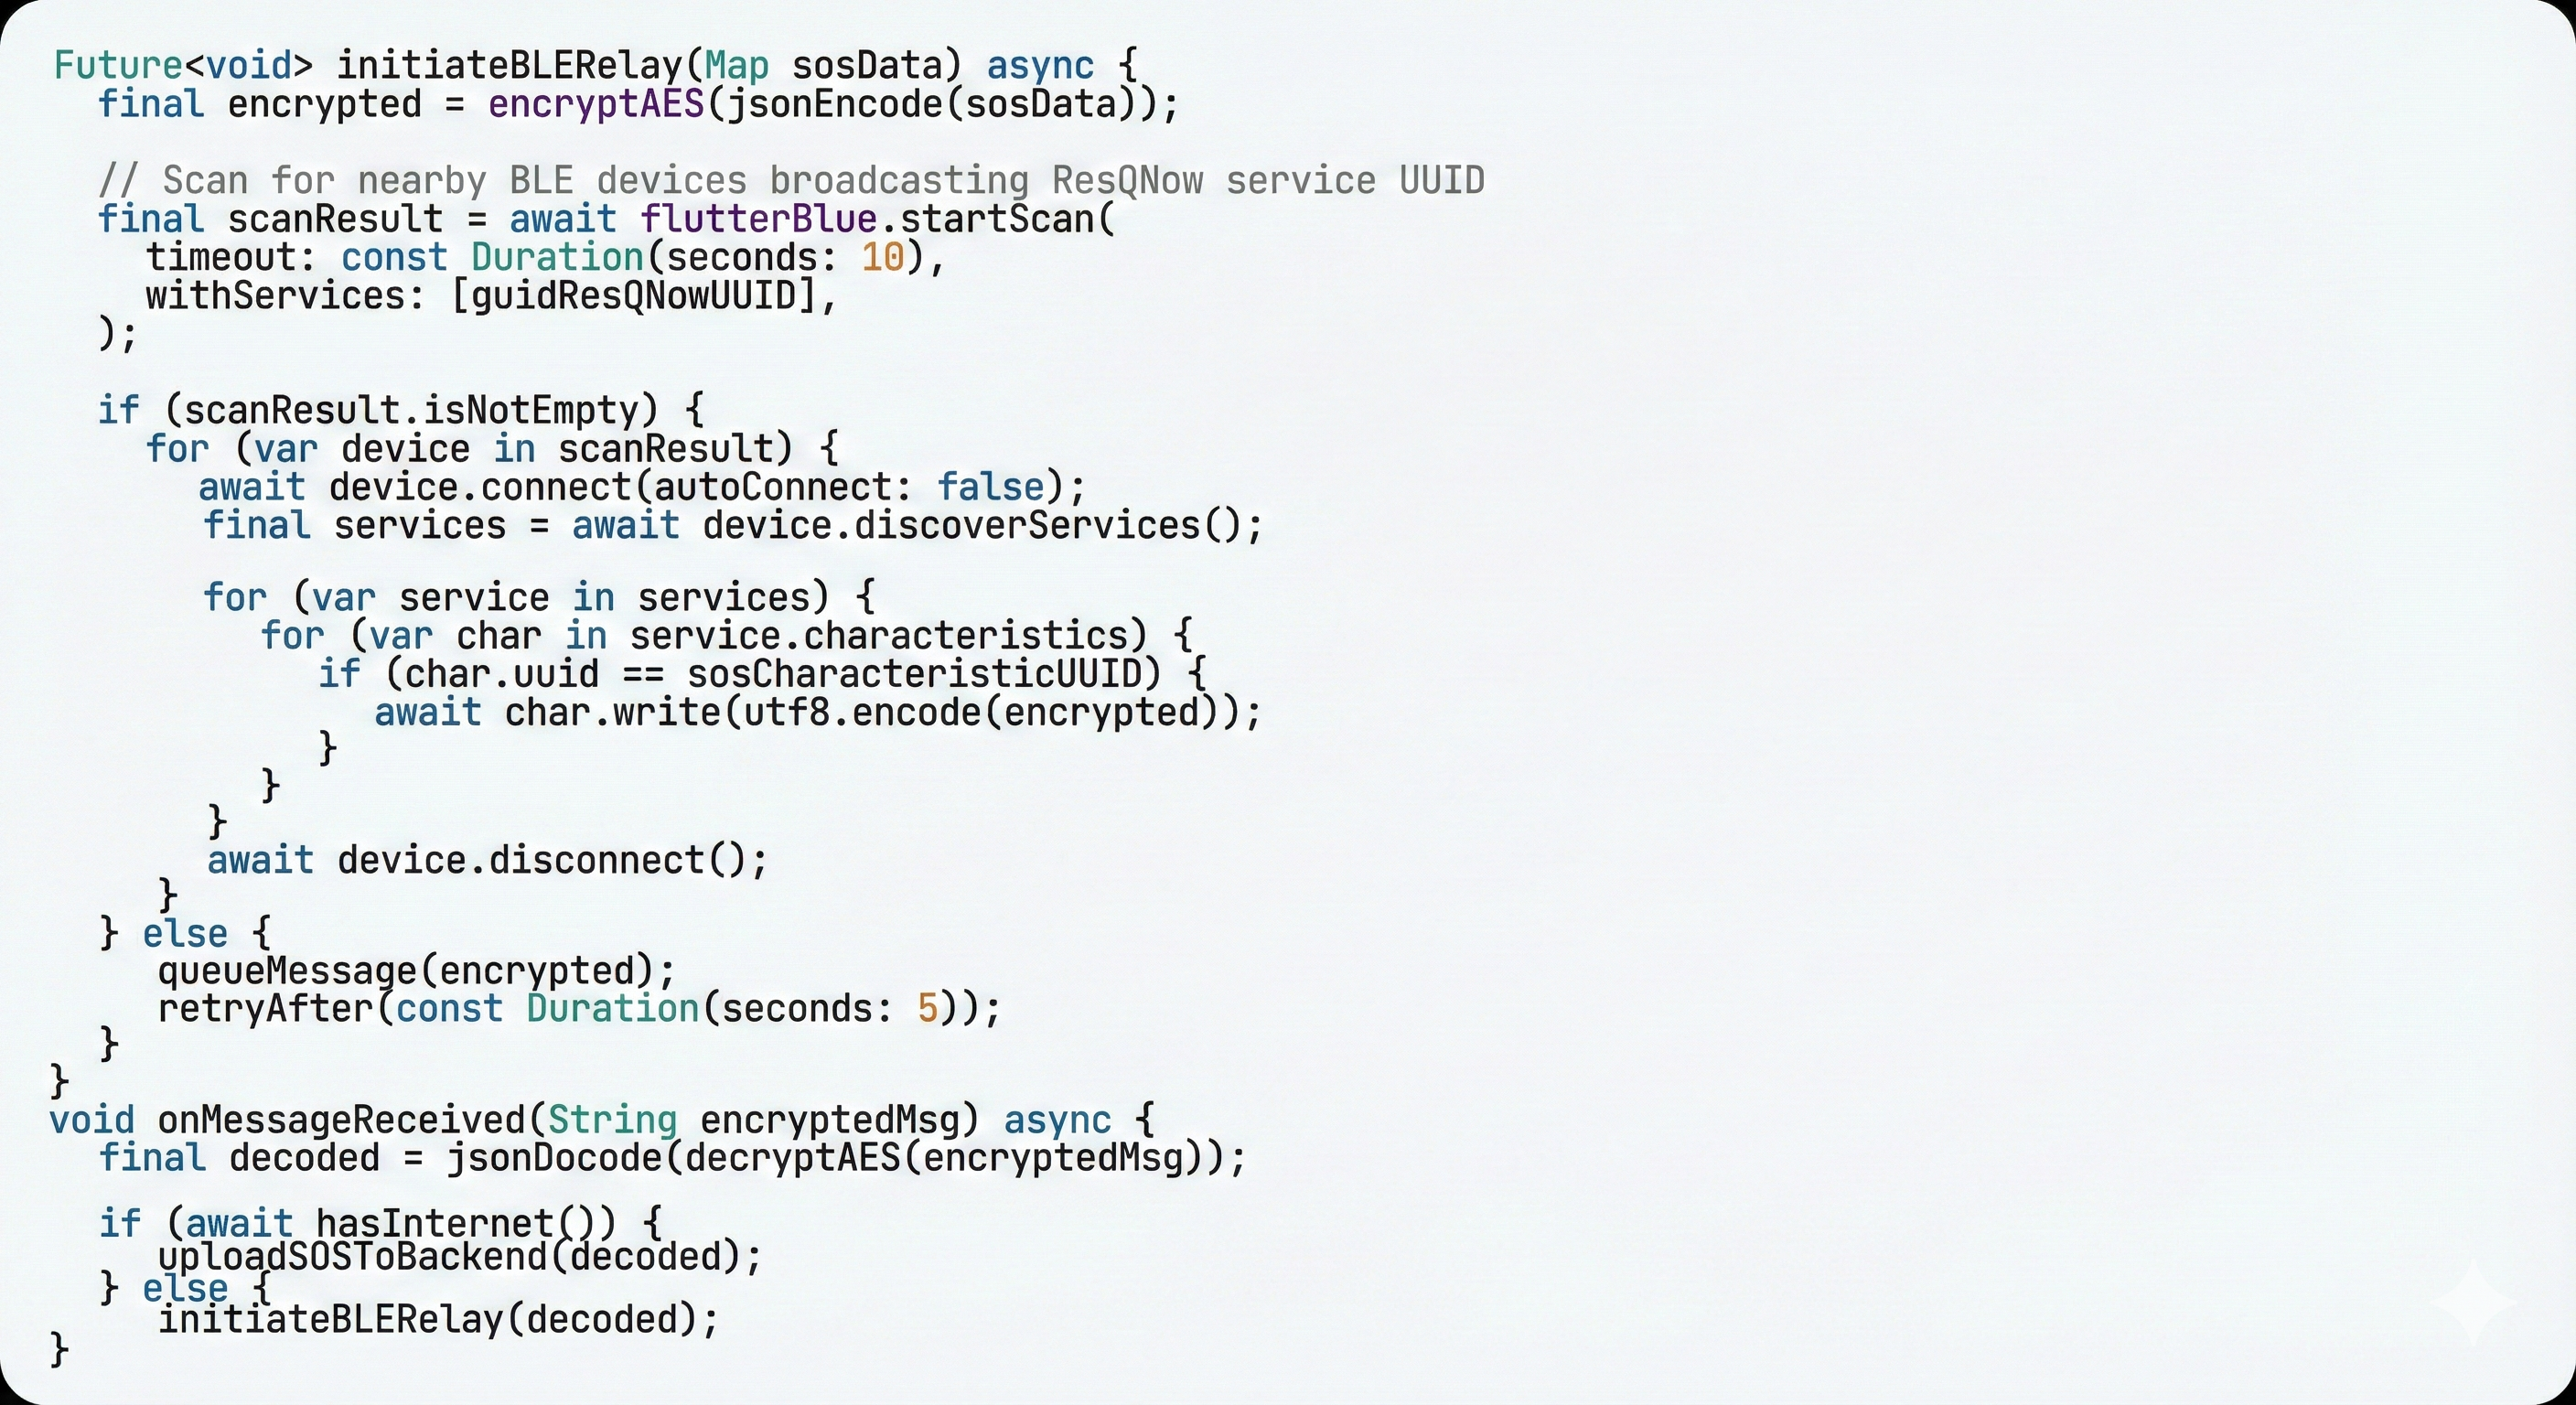
\includegraphics[width=0.95\textwidth]{chapters/ble_code.png}
    \caption{BLE relay implementation with AES encryption, device scanning, and mesh relay logic}
    \label{fig:ble_code}
\end{figure}

% -----------------------------------------------------------------------------
\section{AI-Based Emergency Classification Implementation}

Artificial Intelligence enables ResQNow to automatically analyze user inputs and prioritize emergency handling based on severity and type. The system employs a hybrid approach combining cloud-based AI for detailed analysis and rule-based logic for offline scenarios.

\subsection{AI Classification Pseudocode}

The AI classification process begins by checking network availability to determine which classification method to use. When online, the system sends the user's emergency description to a cloud AI service (Google Gemini or OpenAI GPT) via API call. The response is parsed to extract the predicted emergency type (cardiac arrest, severe bleeding, burn injury, fracture, or general emergency) and severity level (HIGH, MODERATE, or LOW). If the AI returns a confidence score below 0.7, indicating uncertainty, the system supplements or overrides the result using rule-based fallback logic. When offline, the system relies entirely on rule-based classification, which extracts keywords from the user input and matches them against predefined patterns. Keywords like "unconscious" or "not breathing" trigger HIGH severity cardiac arrest classification, while "bleeding" triggers severe bleeding, and so on. Algorithm~\ref{alg: ai_classification} outlines this process. 

\begin{algorithm}[H]
\caption{AI-Based Emergency Classification}
\label{alg: ai_classification}
\begin{algorithmic}[1]
\State \textbf{Input:} User description of emergency (text or voice)
\State \textbf{Output:} Emergency type and severity level
\State
\Procedure{ClassifyEmergency}{$userInput$}
    \If{InternetAvailable()}
        \State $aiResponse \gets$ \Call{CloudAIClassification}{$userInput$}
        \State $emergencyType \gets$ \Call{ExtractType}{$aiResponse$}
        \State $severity \gets$ \Call{ExtractSeverity}{$aiResponse$}
        \State
        \If{$aiResponse.confidence < 0.7$}
            \State $severity \gets$ \Call{RuleBasedFallback}{$userInput$}
        \EndIf
    \Else
        \State $emergencyType \gets$ \Call{RuleBasedClassification}{$userInput$}
        \State $severity \gets$ \Call{RuleBasedSeverity}{$userInput$}
    \EndIf
    \State
    \State \Return \{type: $emergencyType$, severity: $severity$\}
\EndProcedure
\State
\Procedure{RuleBasedClassification}{$userInput$}
    \State $keywords \gets$ \Call{ExtractKeywords}{$userInput$}
    \State
    \If{"unconscious" OR "not breathing" in $keywords$}
        \State \Return \{type: "cardiac\_arrest", severity: "HIGH"\}
    \ElsIf{"bleeding" OR "blood" in $keywords$}
        \State \Return \{type: "severe\_bleeding", severity: "HIGH"\}
    \ElsIf{"burn" in $keywords$}
        \State \Return \{type: "burn\_injury", severity: "MODERATE"\}
    \ElsIf{"fracture" OR "broken" in $keywords$}
        \State \Return \{type: "fracture", severity: "MODERATE"\}
    \Else
        \State \Return \{type: "general\_emergency", severity: "LOW"\}
    \EndIf
\EndProcedure
\end{algorithmic}
\end{algorithm}

\subsection{AI Chatbot Implementation Code}

The following code snippet implements the AI-powered emergency chatbot using Google Gemini API. The \texttt{AIChatService} class maintains conversation history as a list of message objects to enable multi-turn interactions. The \texttt{classifyEmergency()} function constructs a prompt that includes the system instruction (defining the AI's role as an emergency classifier), conversation history for context, and the current user message. It sends an HTTP POST request to the Gemini API endpoint with the API key and receives a JSON response containing the generated text, confidence score, and extracted emergency details. The \texttt{parseResponse()} method uses regular expressions to extract emergency type and severity from the AI's natural language response. The \texttt{ruleBasedFallback()} function implements keyword matching using a Map of emergency keywords to classification results, iterating through the user input to find matches. Error handling includes API timeout (30 seconds), rate limiting with exponential backoff, and automatic fallback to rule-based classification on any API failure. Figure~\ref{fig:ai_code} presents this implementation. 

\begin{figure}[H]
    \centering
    \includegraphics[width=0.95\textwidth]{chapters/ai_code.png}
    \caption{AI chatbot implementation with Gemini API integration, conversation management, and rule-based fallback}
    \label{fig:ai_code}
\end{figure}

% -----------------------------------------------------------------------------
\section{Emergency Contact Notification Implementation}

The notification system ensures reliable alert delivery to emergency contacts through multiple redundant channels. 

\subsection{Multi-Channel Notification Pseudocode}

The notification dispatch mechanism retrieves the list of emergency contacts associated with the user who triggered the SOS alert. It generates a Google Maps URL containing the emergency location coordinates for easy navigation.  A notification message is constructed containing the severity level and location link.  For each emergency contact, the system sends notifications through three channels: push notification via Firebase Cloud Messaging using the contact's device token, SMS via Twilio API using the contact's phone number, and email via SendGrid API using the contact's email address. This multi-channel approach maximizes the probability of successful alert delivery even if one channel fails. Algorithm~\ref{alg:notification} describes this mechanism.

\begin{algorithm}[H]
\caption{Multi-Channel Emergency Notification}
\label{alg:notification}
\begin{algorithmic}[1]
\State \textbf{Input:} SOS alert data, emergency contact list
\State \textbf{Output:} Notifications sent via multiple channels
\State
\Procedure{NotifyEmergencyContacts}{$sosData$}
    \State $contacts \gets$ \Call{GetEmergencyContacts}{$sosData. userId$}
    \State $locationURL \gets$ \Call{GenerateMapURL}{$sosData.latitude$, $sosData.longitude$}
    \State $message \gets$ "Emergency Alert: " + $sosData.severity$ + " at " + $locationURL$
    \State
    \For{each $contact$ in $contacts$}
        \State \Call{SendPushNotification}{$contact. deviceToken$, $message$}
        \State \Call{SendSMS}{$contact.phoneNumber$, $message$}
        \State \Call{SendEmail}{$contact. email$, "Emergency Alert", $message$}
    \EndFor
    \State
    \State \Call{LogNotificationStatus}{$sosData. id$, "notifications\_sent"}
\EndProcedure
\end{algorithmic}
\end{algorithm}

% -----------------------------------------------------------------------------
\section{Responder Acknowledgment Implementation}

The responder acknowledgment system enables nearby users to acknowledge emergency alerts while preventing duplicate responses through atomic database transactions.

\subsection{Responder Acknowledgment Pseudocode}

The acknowledgment workflow uses database transactions to handle concurrent acknowledgment attempts. When a responder attempts to claim an emergency, the system begins a Firestore transaction and retrieves the current SOS alert document. It checks whether another responder has already claimed the alert by examining the responderId field.  If the field is not null, the transaction is rolled back and an error message is returned. Otherwise, the system updates the alert with the responder's ID, name, response timestamp, and changes the status to "ACKNOWLEDGED". The transaction is committed atomically, ensuring that only one responder can successfully claim each emergency even under concurrent access. Finally, the original alert sender is notified that help is on the way.  Algorithm~\ref{alg:responder} outlines this workflow.

\begin{algorithm}[H]
\caption{Responder Acknowledgment with Concurrency Control}
\label{alg: responder}
\begin{algorithmic}[1]
\State \textbf{Input:} SOS alert ID, responder user ID
\State \textbf{Output:} Acknowledgment status (success or already taken)
\State
\Procedure{AcknowledgeEmergency}{$sosId$, $responderId$}
    \State \Call{BeginTransaction}{}
    \State $sosAlert \gets$ \Call{GetSOSAlert}{$sosId$}
    \State
    \If{$sosAlert.responderId \neq null$}
        \State \Call{RollbackTransaction}{}
        \State \Return "Already acknowledged by another responder"
    \EndIf
    \State
    \State $sosAlert.responderId \gets$ $responderId$
    \State $sosAlert.responseTimestamp \gets$ \Call{GetCurrentTimestamp}{}
    \State $sosAlert.status \gets$ "ACKNOWLEDGED"
    \State
    \State \Call{UpdateSOSAlert}{$sosAlert$}
    \State \Call{CommitTransaction}{}
    \State \Call{NotifyOriginator}{$sosId$, $responderId$}
    \State
    \State \Return "Acknowledgment successful"
\EndProcedure
\end{algorithmic}
\end{algorithm}

% -----------------------------------------------------------------------------
\section{GPS Location Tracking Implementation}

Accurate location tracking is critical for emergency response coordination.  The GPS module continuously monitors device location and provides real-time updates during active emergencies.

\subsection{Location Tracking Pseudocode}

The location tracking mechanism initializes by requesting location permission from the user.  Upon permission grant, the system starts a location stream that continuously monitors GPS coordinates. Each location update triggers the \texttt{OnLocationUpdate} procedure, which extracts latitude, longitude, and accuracy values. If an emergency is currently active, the system updates the SOS document in Firestore with the new coordinates and notifies emergency contacts of the location change, enabling real-time tracking.  The location is also cached locally for offline use, ensuring that the most recent known position is available even without GPS signal. Algorithm~\ref{alg:gps} describes this mechanism.

\begin{algorithm}[H]
\caption{Continuous GPS Location Tracking}
\label{alg:gps}
\begin{algorithmic}[1]
\State \textbf{Input:} Location permission granted
\State \textbf{Output:} Real-time GPS coordinates
\State
\Procedure{InitializeLocationTracking}{}
    \State \Call{RequestLocationPermission}{}
    \If{PermissionGranted()}
        \State \Call{StartLocationStream}{}
    \Else
        \State \Call{ShowPermissionError}{}
    \EndIf
\EndProcedure
\State
\Procedure{OnLocationUpdate}{$location$}
    \State $latitude \gets$ $location. latitude$
    \State $longitude \gets$ $location.longitude$
    \State
    \If{EmergencyActive()}
        \State \Call{UpdateSOSLocation}{$latitude$, $longitude$}
        \State \Call{NotifyContactsOfLocationUpdate}{$latitude$, $longitude$}
    \EndIf
    \State \Call{CacheLocation}{$latitude$, $longitude$}
\EndProcedure
\end{algorithmic}
\end{algorithm}

% ----------------------------------------------------------------------------- 

}
\input{chapters/chapter6.tex}
\input{chapters/chapter7.tex}
\input{chapters/chapter8.tex}
\input{chapters/chapter9.tex}

%\addcontentsline{toc}{chapter}{References} % Adding References to the ToC
\
\end{document}
